\documentclass[sans,14pt]{beamer}
\usepackage{pgfpages}
%\setbeameroption{show notes on second screen}
%\setbeameroption{show notes}
\setbeameroption{hide notes}

\usepackage{etex}


\usepackage{fixltx2e} % for \textsubscript


%% Format the bibliography
\usepackage[backend=bibtex,style=alphabetic]{biblatex}
\addbibresource{references}
\setbeamercolor*{bibliography entry title}{fg=MyDarkGrey}
\setbeamercolor*{bibliography entry author}{fg=black}
\setbeamercolor*{bibliography entry location}{fg=black}
\setbeamercolor*{bibliography entry note}{fg=black}
\setbeamertemplate{bibliography item}[text]

% Space between label and reference
\setlength{\biblabelsep}{-15pt}


\mode<presentation>
{
  \usetheme{Copenhagen}
  \usecolortheme{beaver}
  \usefonttheme[onlymath]{serif}
}

%% Change bullet points style
%\setbeamertemplate{itemize items}[triangle]
\setbeamertemplate{itemize items}{{\textemdash}}
\setbeamercolor*{item}{fg=MyDarkGrey}

%% Remove navigation symbols
\setbeamertemplate{navigation symbols}{}
\setbeamertemplate{headline}{}

%% Use only frame number (no total frame count) in footer
\setbeamertemplate{footline}{%
  \raisebox{5pt}{\makebox[\paperwidth]{\hfill\makebox[20pt]{
        \scriptsize\insertframenumber}}}
}

% Adjust margin of itemize environment
\setlength{\leftmargini}{0pt}
\setlength{\leftmarginii}{10pt}
\setlength{\leftmarginiii}{17pt}

%% Adjust font sizes
\setbeamerfont{frametitle}{size=\Large}
\setbeamerfont{normal text}{size=\small}
\setbeamerfont{itemize/enumerate body}{size=\small}
\setbeamerfont{itemize/enumerate subbody}{size=\small}
\setbeamerfont{itemize/enumerate subsubbody}{size=\footnotesize}

%%% To use the Cabin-Condensed fonts
%%% More fonts: see http://www.tug.dk/FontCatalogu
% \usepackage[latin1]{inputenc}
% \usepackage[T1]{fontenc}
% \usepackage[sfdefault]{cabin} 
\usepackage{PTSans} 
\usepackage{PTSansNarrow} 
\renewcommand*\familydefault{\sfdefault} %% Only if the base font of the document is to be sans serif
\usepackage[T1]{fontenc}

\newenvironment{ptnormal}{\fontfamily{PTSans-TLF}\selectfont}{\par}


\usepackage{amsmath}
\usepackage{amsfonts}
\usepackage{amssymb}
\usepackage{amsthm}
\usepackage{bm}
\usepackage{booktabs}
\usepackage{color}
\usepackage{epstopdf}
\usepackage{fancyhdr}
\usepackage{fancybox}
\usepackage[all]{xy}
\usepackage{graphicx}
\usepackage{multirow}
\usepackage[normalem]{ulem}
\usepackage{url}
\usepackage{dsfont}
%


% tikzmark command, for shading over items
\usepackage{tikz}
\usetikzlibrary{calc}
\newcommand{\tikzmark}[1]{\tikz[overlay,remember picture] \node (#1) {};}
\usetikzlibrary{decorations.pathreplacing} % for curly braces
\usepackage[framemethod=tikz]{mdframed} % for fancy title page and other boxes

%% Subfigures
\usepackage[labelformat=simple,caption=false,textfont=scriptsize]{subfig}
\renewcommand{\thesubfigure}{\relax} % do not number captions of
                                     % subfloats


%% to write text at the bottom of a beamer slide
%\def\writeatbottom#1{\vskip 0pt plus 1filll \scriptsize #1}

\newcommand{\topspace}{\rule{0pt}{2.6ex}}
\newcommand{\botspace}{\rule[-1.2ex]{0pt}{0pt}}


%%% Colors
%\usepackage{color}
\definecolor{MyBlue}{rgb}{0.27,0.62,0.73}%{0.,0.2,0.4} 
\definecolor{Aubergine}{rgb}{0.47,0.13,0.44} % 119 33 111
\definecolor{MyTurq}{rgb}{0.,0.8,0.8} 
\definecolor{MyDarkGrey}{rgb}{0.3,0.3,0.3} 
\definecolor{MyMedGrey}{rgb}{0.6,0.6,0.6} 
\definecolor{MyLightGrey}{rgb}{0.95,0.95,0.95} 
\definecolor{MyDarkRed}{rgb}{0.8,0.,0.} 
\definecolor{MyOrange}{rgb}{0.93,0.56,0.25}
\definecolor{MyPink}{rgb}{0.73,0.27,0.39}
\definecolor{MyLightYellow}{HTML}{FFFFCC}
%\usepackage[colorlinks=true,citecolor=MyTurq]{hyperref}
\AtEveryCite{\color{MyMedGrey}}

\newcommand{\blue}[1]{{\color{MyBlue}{\textbf{#1}}}}
\newcommand{\red}[1]{{\color{MyOrange}{\textbf{#1}}}}
\newcommand{\black}[1]{{\color{MyDarkGrey}{\textbf{#1}}}}
\newcommand{\yellow}[1]{{\color{MyLightYellow}{\textbf{#1}}}}

\newcommand{\TODO}{{\color{MyDarkRed}{TODO~}}}

\setbeamercolor{normal text}{fg=MyDarkGrey}
\setbeamercolor{frametitle}{fg=Aubergine}

%%% ---- Titre des slides  (underline) ----------------
\setbeamertemplate{frametitle}{%
    \usebeamerfont{frametitle}\insertframetitle\strut%
    \vskip-.05\baselineskip%
    \leaders\vrule width \paperwidth\vskip1.pt%
    \vskip0pt%
    \nointerlineskip
}
%%% ---------------------------------------------------


% --- Math symbols -------------------------------------------------------------
\newcommand{\EE}{{\mathbb E}}
\newcommand{\PP}{{\mathbb P}}
\newcommand{\NN}{{\mathbb N}}
\newcommand{\RR}{{\mathbb R}}

\newcommand{\avec}{\vec{a}}
\newcommand{\alphavec}{\vec{\alpha}}
\newcommand{\betavec}{\vec{\beta}}
\newcommand{\cvec}{\vec{c}}
\newcommand{\fvec}{\vec{f}}
\newcommand{\muvec}{\vec{\mu}}
\newcommand{\mvec}{\vec{m}}
\newcommand{\rvec}{\vec{r}}
\newcommand{\thetavec}{\vec{\theta}}
\newcommand{\xvec}{\vec{x}}
\newcommand{\yvec}{\vec{y}}
\newcommand{\wvec}{\vec{w}}
\newcommand{\uvec}{\vec{u}}
\newcommand{\vvec}{\vec{v}}
\newcommand{\zvec}{\vec{z}}

% \newcommand{\amat}{{\mathbf A}}}
% \newcommand{\dmat}{{\mathbf D}}
% \newcommand{\gmat}{{\mathbf G}}
% \newcommand{\kmat}{{\mathbf K}}
% \newcommand{\lmat}{{\mathbf L}}
% \newcommand{\mmat}{{\mathbf M}}
% \newcommand{\wmat}{{\mathbf W}}
% \newcommand{\xmat}{{\mathbf X}}

\newcommand{\aset}{\mathcal{A}}
\newcommand{\cset}{\mathcal{C}}
\newcommand{\dset}{\mathcal{D}}
\newcommand{\fcal}{\mathcal{F}}
\newcommand{\hcal}{\mathcal{H}}
\newcommand{\ncal}{\mathcal{N}}
\newcommand{\nset}{\mathcal{N}}
\newcommand{\rcal}{\mathcal{R}}
\newcommand{\sset}{\mathcal{S}}
\newcommand{\vset}{\mathcal{V}}
\newcommand{\tset}{\mathcal{T}}
\newcommand{\xcal}{\mathcal{X}}
\newcommand{\ycal}{\mathcal{Y}}

\newcommand{\lzeronorm}[1]{\left|\left|#1\right|\right|_0}
\newcommand{\lonenorm}[1]{\left|\left|#1\right|\right|_1}
\newcommand{\ltwonorm}[1]{\left|\left|#1\right|\right|_2}

\usepackage{bbm}
\newcommand{\indic}{\mathbbm{1}}

\DeclareMathOperator*{\argmin}{arg\,min}
\DeclareMathOperator*{\argmax}{arg\,max}
\graphicspath{{./figures/}}

% ------------------------------------------------------------------------------



% \newcommand{\source}[1]{\begin{textblock*}{4cm}(8.7cm,8.6cm)
%     \begin{beamercolorbox}[ht=0.5cm,right]{framesource}
%       \usebeamerfont{framesource}\usebeamercolor[fg]{framesource} Credits: {#1}
%     \end{beamercolorbox}
% \end{textblock*}}




\newcommand{\mytitle}{Fondamentaux du Machine Learning}
\author[Walter]{Thomas Walter \and  Chlo\'e-Agathe~Azencott \and Florian Massip} 
\institute[CBIO]{\inst{1} Centre for Computational Biology(CBIO), Mines Paris, PSL University\and %
                      \inst{2} Institut Curie\and
                      \inst{3} U1331 - INSERM}

\date{\small \today}

\begin{document}
{

  \begin{frame}[plain]
    \fontfamily{PTSansNarrow-TLF}\selectfont
    \begin{center}
      {\ptnormal{\textit{Formation Chef de Projet IA}}}
    \end{center}

    \vspace{70pt}

    \centerline{{\Large \bf \mytitle}}

    \vspace{15pt}

    \centerline{\insertauthor}

    \vspace{15pt}

    {\footnotesize
      \centerline{Center for Computational Biology (CBIO)}
    
      \centerline{Mines Paris -- Institut Curie -- INSERM U900}

      \centerline{PSL Research University \& PR[AI]RIE, Paris, France}
    }

    \centerline {\insertdate}

\end{frame}

% Do not count title slide when numbering frames
\addtocounter{framenumber}{-1}


% Overview
\begin{frame}
  \frametitle{Programme}

  \begin{itemize}
  \item Introduction à l'apprentissage automatique
  \item \blue{Cours 1 :} Minimisation du risque empirique 
  \item \blue{Cours 2 :} Régularisation et sélection de modèle
  \item \blue{Cours 3 :} Arbres et méthodes ensemblistes
  \item \blue{Cours 4 :} Méthodes à noyaux 
  \item \blue{Cours 5 :} Réduction de dimension
  \item \blue{Cours 6 :} Clustering
  \item Travaux pratiques : mise en œuvre des notions et algorithmes avec scikit-learn (Python numérique).
\end{itemize}
\end{frame}




\begin{frame}
  \begin{center}
    \large{1. Noyaux}
  \end{center}
\end{frame}

\begin{frame}
  \frametitle{1.1 Produit scalaire}
  \begin{itemize}
  \item $\langle \xvec, \xvec^\prime \rangle = \sum_{j=1}^p x_j x_j^\prime$
  \item $\langle \xvec, \xvec^\prime \rangle = \ltwonorm{\xvec} \ltwonorm{\xvec^\prime} \cos \theta$ \hspace{1em}
     $\ltwonorm{\xvec}^2 = \langle \xvec, \xvec \rangle$
  \item Interprétable comme \blue{mesure de similarité}
  \item \blue{Forme définie positive bilinéaire :}
    \begin{itemize}
    \item $\langle \xvec, \xvec^\prime \rangle = \langle \xvec^\prime, \xvec \rangle$
      pour tout $\xvec, \xvec^\prime \in \mathcal{X}$
    \item $\langle \xvec + \zvec, \xvec^\prime \rangle = \langle \xvec, \xvec^\prime \rangle +
      \langle \zvec, \xvec^\prime \rangle$       pour tout $\xvec, \xvec^\prime, \zvec \in \mathcal{X}$
    \item $\langle a \xvec, \xvec^\prime \rangle = a \langle \xvec, \xvec^\prime \rangle$ pour tout $a \in \RR$
    \item $\langle \xvec, \xvec \rangle \geq 0$ et $\langle \xvec, \xvec \rangle = 0 \text{ ssi } \xvec = 0$
    \end{itemize}
  \item Apparaît dans de nombreux algorithmes d'apprentissage.
  \end{itemize}
\end{frame}

\begin{frame}
  \frametitle{1.2 Noyau}
  \begin{itemize}
  \item \blue{Généralisation} du produit scalaire : $k: \xcal \times \xcal \rightarrow \RR$
    \begin{itemize}
    \item \blue{sémantiquement} une similarité
    \item \blue{mathématiquement} une forme définie positive 
    \end{itemize}
  \item Aronszajn: Si $k$ est semi-définie positive\footnote{Pour tout
      $m \in \NN^*$, pour tout
      $\{\xvec_1, \xvec_2, \dots, \xvec_m\} \in \xcal,$ la matrice
      $K \in \RR^{m \times m}$ telle que $K_{il} = k(\xvec_i, \xvec_l)$ est
      semi-définie positive}, il existe un espace de Hilbert $\hcal$ et une application
    $\varphi: \xcal \rightarrow \hcal$ telle que
    $\textcolor{MyOrange}{k(\xvec, \xvec^\prime) = \langle \varphi(\xvec), \varphi(\xvec^\prime)\rangle_{\hcal}}$
    pour tout $\xvec, \xvec^\prime, \zvec \in \mathcal{X}$
  \end{itemize}
\end{frame}

\begin{frame}
  \frametitle{1.3 Astuce du noyau}
  \begin{itemize}
    \item[]    $\textcolor{MyOrange}{k(\xvec, \xvec^\prime) = \langle \varphi(\xvec), \varphi(\xvec^\prime)\rangle_{\hcal}}$
    \item Si un algorithme ne fait intervenir les éléments de $\xcal$ que dans
      des produits scalaires, \blue{remplacer ces produits scalaires} par $k$ est
      équivalent à appliquer l'algorithme dans $\hcal$ après avoir appliqué
      $\varphi$
    \item Utile \blue{si $k$ est plus simple à calculer que $\varphi$}
      \pause
    \item Exemple : \blue{noyau quadratique}
      $k: (\xvec, \xvec^\prime) \mapsto (1 + \langle \xvec, \xvec^\prime \rangle)^2$
    \item[] Équivaut à $\varphi : (x_1, x_2, \dots, x_p) \mapsto (1, x_1, \dots, x_p,
      x_1^2, x_2^2, \dots, x_p^2, \sqrt{2} x_1 x_2, \dots, \sqrt{2}x_{p-1}x_p).$
  \end{itemize}
\end{frame}

\begin{frame}
  \frametitle{Noyau quadratique}
  \begin{itemize}
  \item[] $k: (\xvec, \xvec^\prime) \mapsto (1 + \langle \xvec, \xvec^\prime \rangle)^2$
  \item[] Équivaut à $\varphi : (x_1, x_2, \dots, x_p) \mapsto (1, x_1, \dots, x_p,
    x_1^2, x_2^2, \dots, x_p^2, \sqrt{2} x_1 x_2, \dots, \sqrt{2}x_{p-1}x_p).$
  \end{itemize}
  \begin{center}
    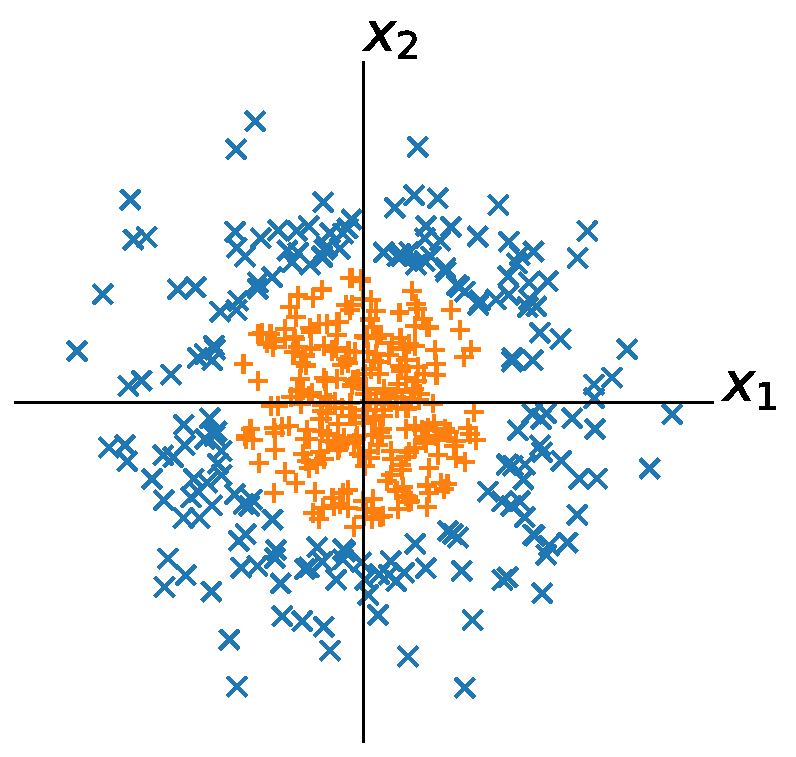
\includegraphics[width=0.4\textwidth]{figures/circular-separable}%
    \hfill
    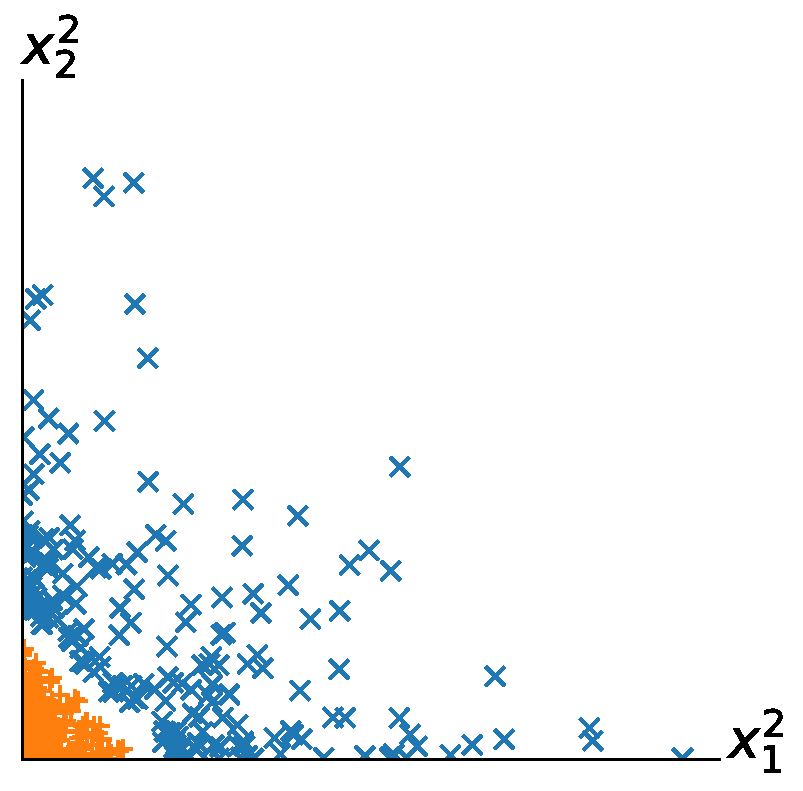
\includegraphics[width=0.4\textwidth]{figures/circular-separable-mapped}%
  \end{center}
\end{frame}

\begin{frame}
  \frametitle{1.4 Régression ridge à noyau}
  \begin{itemize}
  \item \blue{Régression ridge :}
    {\footnotesize $\argmin_{\betavec \in \RR^{p+1}} \frac1n \left(\yvec - X \betavec \right)^\top
      \left(\yvec - X \betavec \right) + \lambda \ltwonorm{\betavec} $}      
    \begin{itemize}
    \item Solution : $\betavec^* = \left(X^\top X + \lambda I_p \right)^{-1} X^\top \yvec$
    \item Modèle : $f: \xvec \mapsto \langle \betavec^*, \xvec \rangle$
    \end{itemize}
  \item Reformulation :
    $f: \xvec \mapsto \textcolor{Aubergine}{\xvec X^\top} \left( \lambda I_n +
      \textcolor{MyPink}{XX^\top} \right)^{-1} \yvec $
    \pause
    \begin{itemize}
    \item $\textcolor{Aubergine}{\xvec X^\top} \in \RR^n$ a pour $i$-ème entrée :
      $\textcolor{Aubergine}{\langle \xvec, \xvec_i \rangle}$    
    \item $\textcolor{MyPink}{X X^\top} \in \RR^{n \times n}$ a pour entrée $(i,l)$ :
      $\textcolor{MyPink}{\langle \xvec_i, \xvec_l \rangle}$
    \end{itemize}
    \pause
  \item \blue{Kernelization :} remplacer $\textcolor{Aubergine}{\xvec X^\top}$ par
    $\textcolor{Aubergine}{\kappa} \in \RR^n$ tel que
    $\textcolor{Aubergine}{\kappa_i = k(\xvec, \xvec_i)}$ et $\textcolor{MyPink}{XX^\top}$ par
    $\textcolor{MyPink}{K} \in \RR^{n \times n}$ telle que $\textcolor{MyPink}{K_{il} = k(\xvec_i, \xvec_l)}$
  \item[] équivaut à transformer les données par $\varphi$ puis apprendre une régression ridge, \blue{pour environ le même coût algorithmique}
  \end{itemize}
\end{frame}

\begin{frame}
  \frametitle{1.5 Exemples de noyaux}
  \begin{itemize}
  \item \blue{Noyau quadratique} $k: (\xvec, \xvec^\prime) \mapsto (1 + \langle \xvec, \xvec^\prime \rangle)^2$
  \item[] $\varphi$ calcule tous les monômes de degré au plus 2 de $x_1, x_2, \dots, x_p$ 
    \pause
  \item \blue{Noyau polynomial} $k: (\xvec, \xvec^\prime) \mapsto (1 + \langle \xvec, \xvec^\prime \rangle)^d$
  \item[] $\varphi$ calcule tous les monômes de degré au plus $d$ de $x_1, x_2, \dots, x_p$ 
    \pause 
  \item \blue{Noyau RBF gaussien} $k: (\xvec, \xvec^\prime) \mapsto
    \exp\left( - \frac{\ltwonorm{\xvec - \xvec^\prime}^2}{\sigma^2} \right)$
  \item[] $\varphi$ calcule tous les monômes de $x_1, x_2, \dots, x_p$ 
  et $\hcal$ est de dimension infinie. 
  \end{itemize}
\end{frame}

\begin{frame}
  \frametitle{1.5 Exemples de noyaux}
  \begin{itemize}
  \item \blue{Noyau pour chaîne de caractères} $k: (\xvec, \xvec^\prime) \mapsto
    \sum_{u \in \aset^m} \psi_u(\xvec) \psi_u(\xvec^\prime)$
    \begin{itemize}
    \item $\aset^m$ = l'ensemble des chaînes de $m$ caractères sur l'alphabet $\aset$
    \item $\psi_u(\xvec) = 1$ si $u$ est une sous-chaîne de $\xvec$ et $0$ sinon.
    \end{itemize}
  \pause
  \item $k(\xvec, \xvec^\prime)$ est le nombre de chaînes de $m$ caractères
    communes à $\xvec$ et $\xvec^\prime$ et peut être calculé en
    $\mathcal{O}(|\xvec|)$ au lieu de $\mathcal{O}(|\aset|^m)$.
    \pause
  \item Si $m=8$, $|\aset|=20$ et en moyenne $|\xvec| = 485,$ on compare 25,6 milliards
    d'opérations à moins de 500.
  \end{itemize}
\end{frame}

\begin{frame}
  \frametitle{Recap : Méthodes à noyau}
  \begin{itemize}
  \item \black{Idée :} Remplacer dans un algorithme tous les \blue{produits scalaires} par des \blue{noyaux}
  \item Apprendre des modèles \blue{non-linéaires} efficacement
  \item Appliquer des modèles linéaires à des \blue{objets} dont la représentation en $p$ dimensions n'est pas évidente (images, protéines, graphes, etc.)
    
  \end{itemize}
\end{frame}

\begin{frame}
  \begin{center}
    \large{2. Machines à vecteurs de support}
  \end{center}
\end{frame}

\begin{frame}[t]
  \frametitle{2.1 Formulation primale}
  \begin{itemize}
  \item Classification binaire, $\ycal = \{-1, 1\}$ 
    \[\argmin_{\betavec \in \RR^p, b \in \RR} \frac12 \ltwonorm{\betavec}^* + C \sum_{i=1}^n
      \max\left( 0, 1 - y_i \left( \langle \betavec, \xvec_i \rangle + b \right)\right)\]
  \end{itemize}
  \begin{center}
    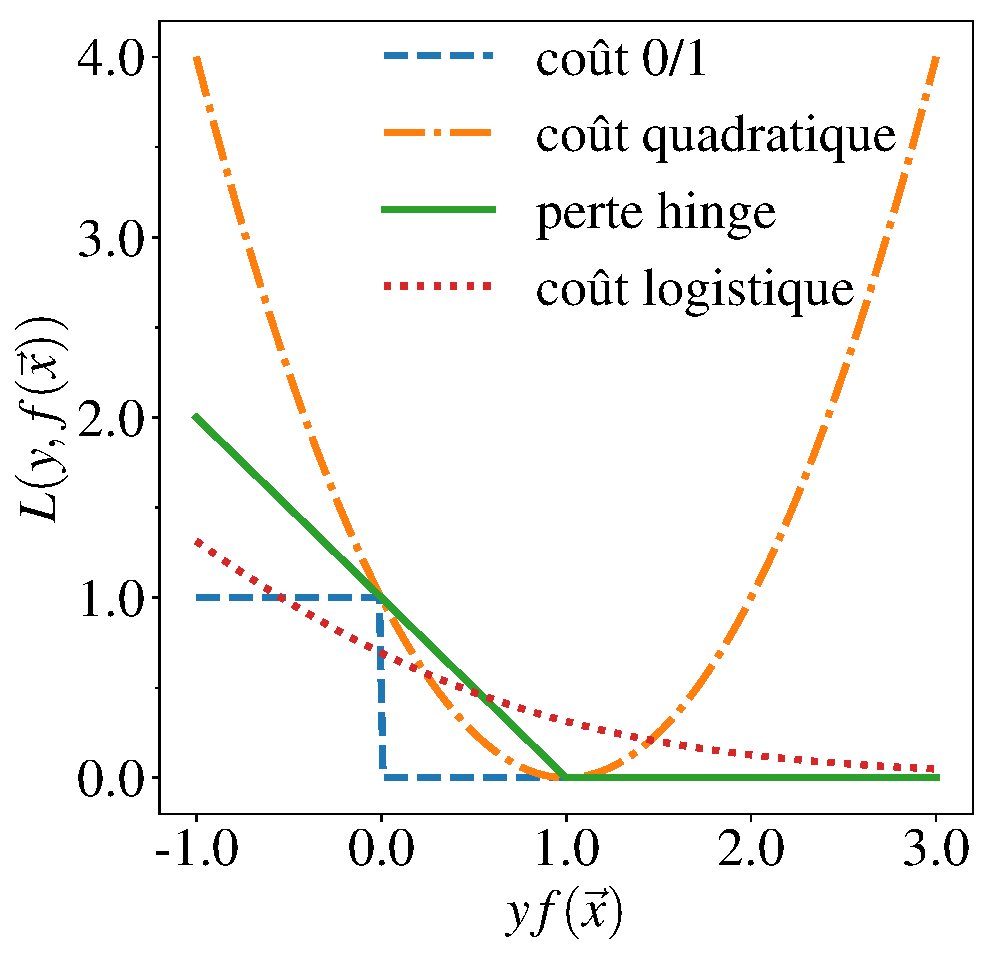
\includegraphics[width=0.5\textwidth]{figures/classif_losses}%
  \end{center}
\end{frame}

\begin{frame}[t]
  \frametitle{2.1 Formulation primale}
  \begin{itemize}
  \item Classification binaire, $\ycal = \{-1, 1\}$ 
    \[\argmin_{\betavec \in \RR^p, b \in \RR} \frac12 \ltwonorm{\betavec}^* + C \sum_{i=1}^n
      \max\left( 0, 1 - y_i \left( \langle \betavec, \xvec_i \rangle + b \right)\right)\]
  \end{itemize}
  \begin{center}
    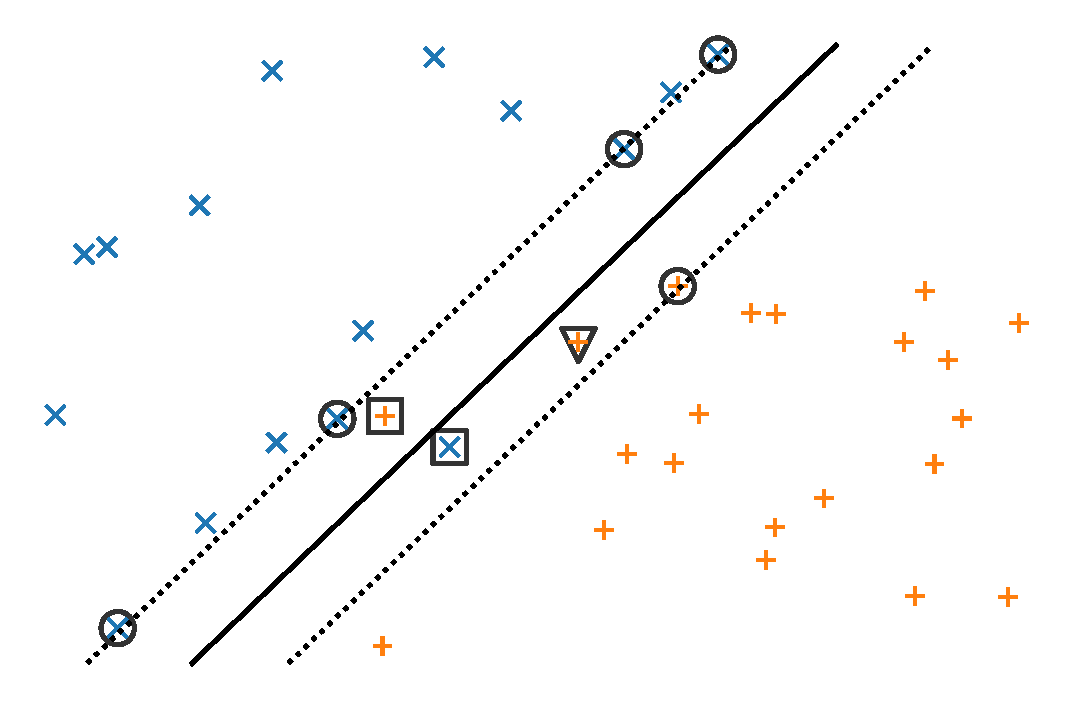
\includegraphics[width=0.7\textwidth]{figures/non-linearly-separable}%
  \end{center}
\end{frame}

\begin{frame}[t]
  \frametitle{2.2 Formulation duale}
    {\small \[\argmax_{\alphavec \in \RR^n} \sum_{i=1}^n \alpha_i - \frac12 \sum_{i=1}^n \sum_{l=1}^n
      \alpha_i \alpha_l y_i y_l \langle \xvec_i, \xvec_l \rangle   \]}
  \begin{itemize}
  \item[] sous les contraintes $\sum_{i=1}^n \alpha_i y_i = 0$  et $0 \leq \alpha_i \leq C$ 
  \item Modèle : $f: \xvec \mapsto \sum_{i=1}^n \alpha_i y_i \langle \xvec_i, \xvec \rangle$
  \end{itemize}
\end{frame}

\begin{frame}[t]
  \frametitle{2.3 SVR (Support Vector Regression)}
  \begin{itemize}
  \item Perte $\varepsilon$-insensible :
    \[L(y, f(\xvec) = \max(0, |f(\xvec) - y| - \varepsilon)\]
  \end{itemize}
  \begin{center}
    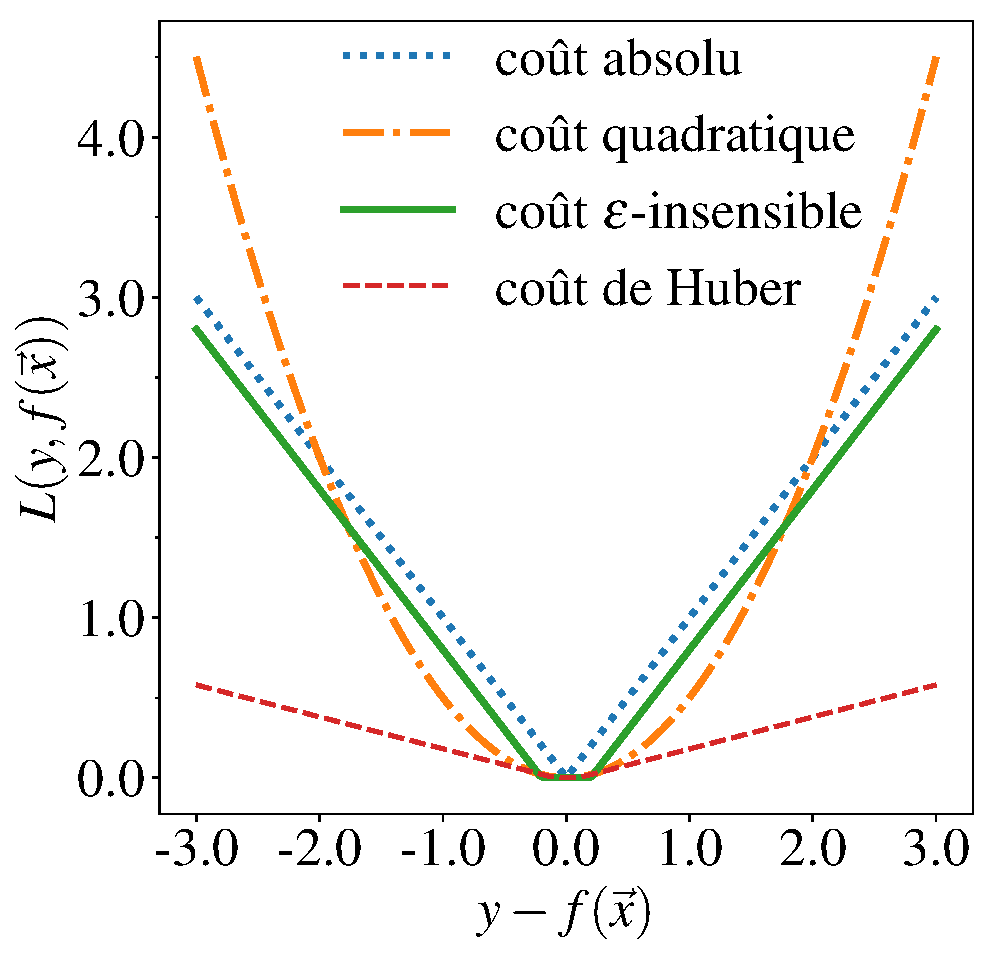
\includegraphics[width=0.5\textwidth]{figures/regression_losses}%
  \end{center}
\end{frame}

\end{document}
